\section{Introducción}
Se busca resolver el siguiente circuito euleriano, el cual se muestra en la 
figura\ref{fig:circuito_euleriano}.

\begin{figure}[H]
    \centering
    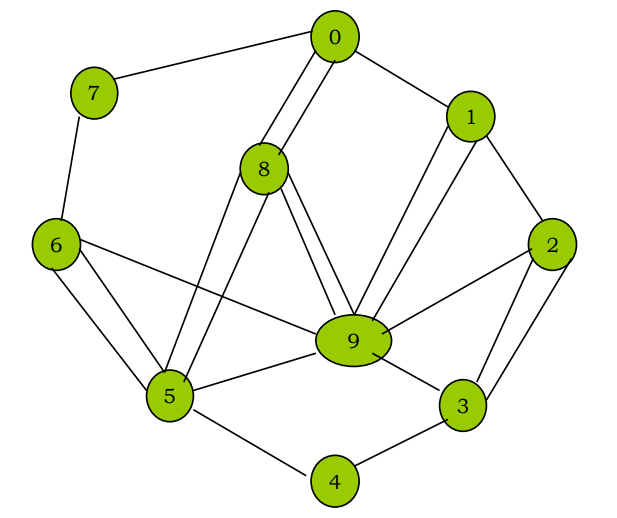
\includegraphics[width=0.5\textwidth]{rsc/img/circuito_euler.png}
    \caption{Circuito Euleriano a resolver.}\label{fig:circuito_euleriano}
\end{figure}

Como primer paso, se debe verificar que el circuito es efectivamente euleriano, 
lo cual se cumple si cada vértice tiene un grado par y el grafo es conexo. En este caso, cada vértice 
del circuito tiene un grado de 2, lo que confirma que el circuito es euleriano.

\begin{table}[H]
    \centering
    \begin{tabular}{|c|c|}
        \hline
        Vértice & Grado \\
        \hline
        0 & 4 \\
        1 & 4 \\
        2 & 4 \\
        3 & 4 \\
        4 & 2 \\
        5 & 6 \\
        6 & 4 \\
        7 & 2 \\
        8 & 6 \\
        9 & 8 \\
        \hline
    \end{tabular}
    \caption{Grados de los vértices del circuito.}\label{tab:grados_vertices}
\end{table}
